%
% introduction.tex
%
% Copyright (C) 2024 by SpaceLab.
%
% EPS 2.0 Qualification Test Plan
%
% This work is licensed under the Creative Commons Attribution-ShareAlike 4.0
% International License. To view a copy of this license,
% visit http://creativecommons.org/licenses/by-sa/4.0/.
%

%
% \brief Product Presentation chapter.
%
% \author Ramon de Araujo Borba <ramonborba97@gmail.com>
%
% \version 0.1.0
%
% \date 2024/02/14
%

\chapter{Hardware Models} \label{ch:product-presentation}

For the execution of this test plan, dedicated qualification models of the EPS 2.0 were manufactured.
\autoref{fig:eps2-pcb-top} and \autoref{fig:eps2-pcb-bottom} show the models as they were delivered to SpaceLab.

\begin{figure}[htp]
    \centering
    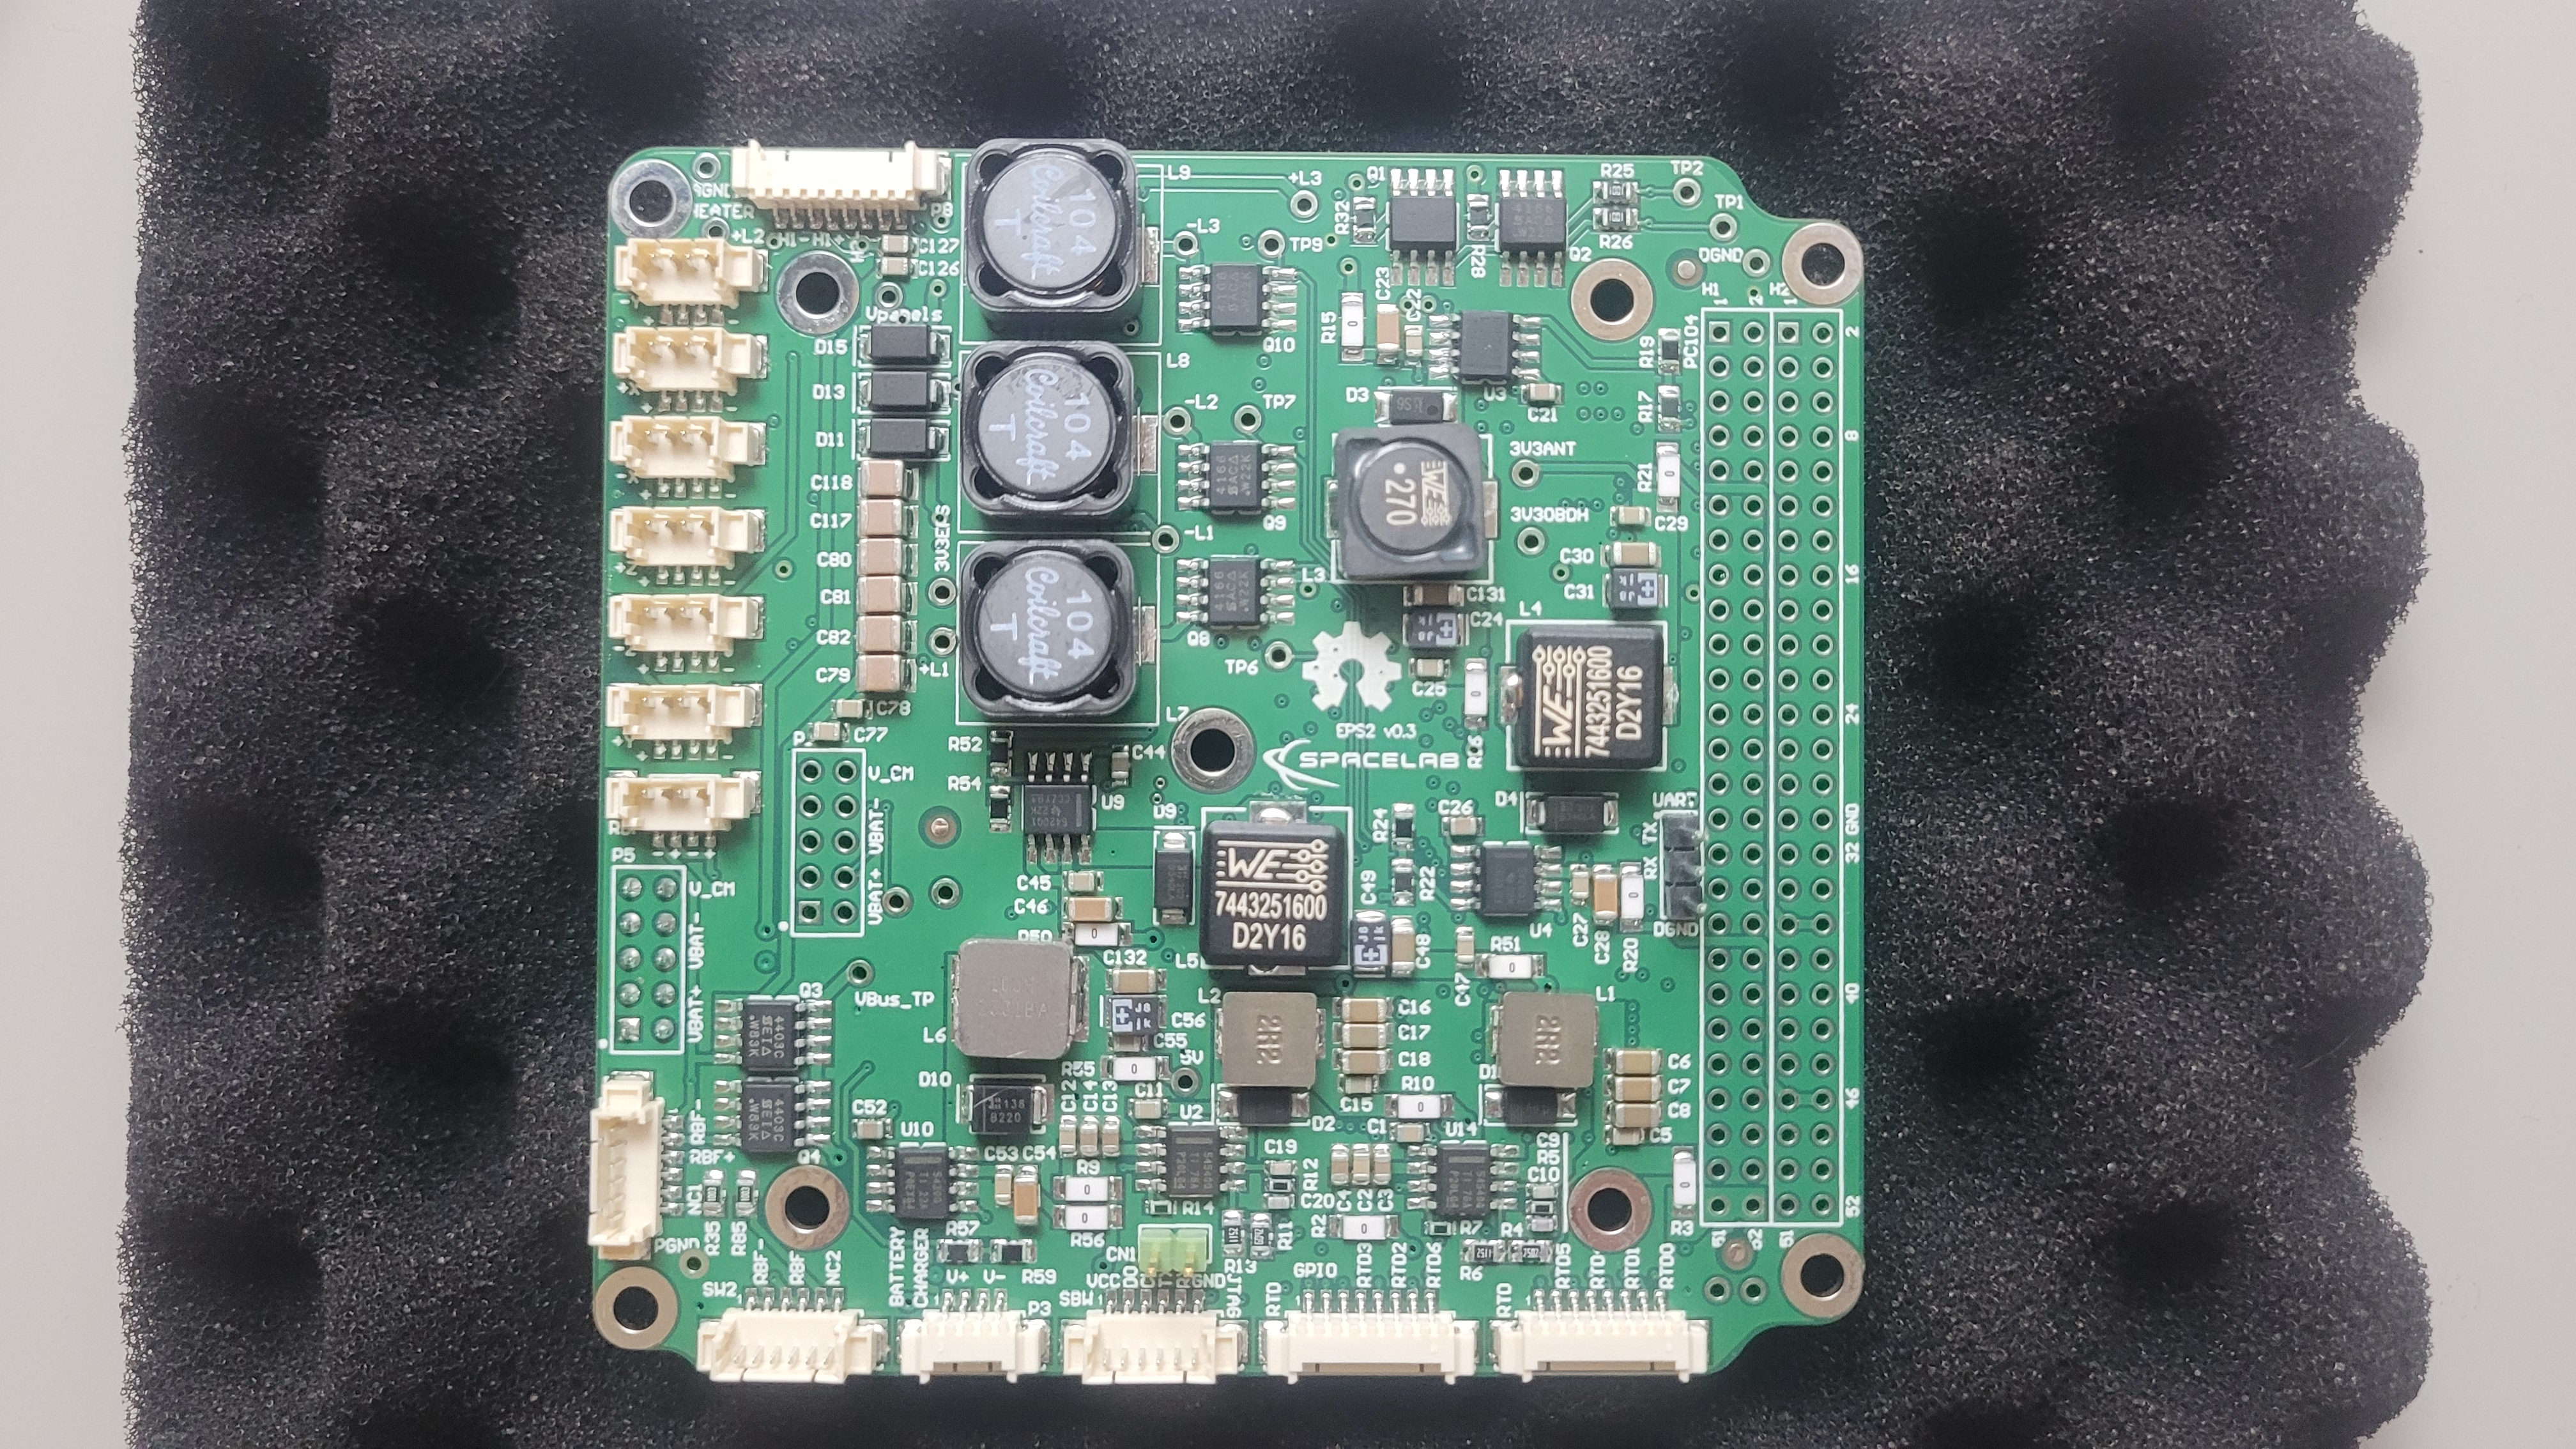
\includegraphics[width=0.6\textwidth, keepaspectratio]{figures/eps2_pcb_top.jpg}
    \caption{EPS 2.0 v0.3 top view.}
    \label{fig:eps2-pcb-top}
\end{figure}


\begin{figure}[htp]
    \centering
    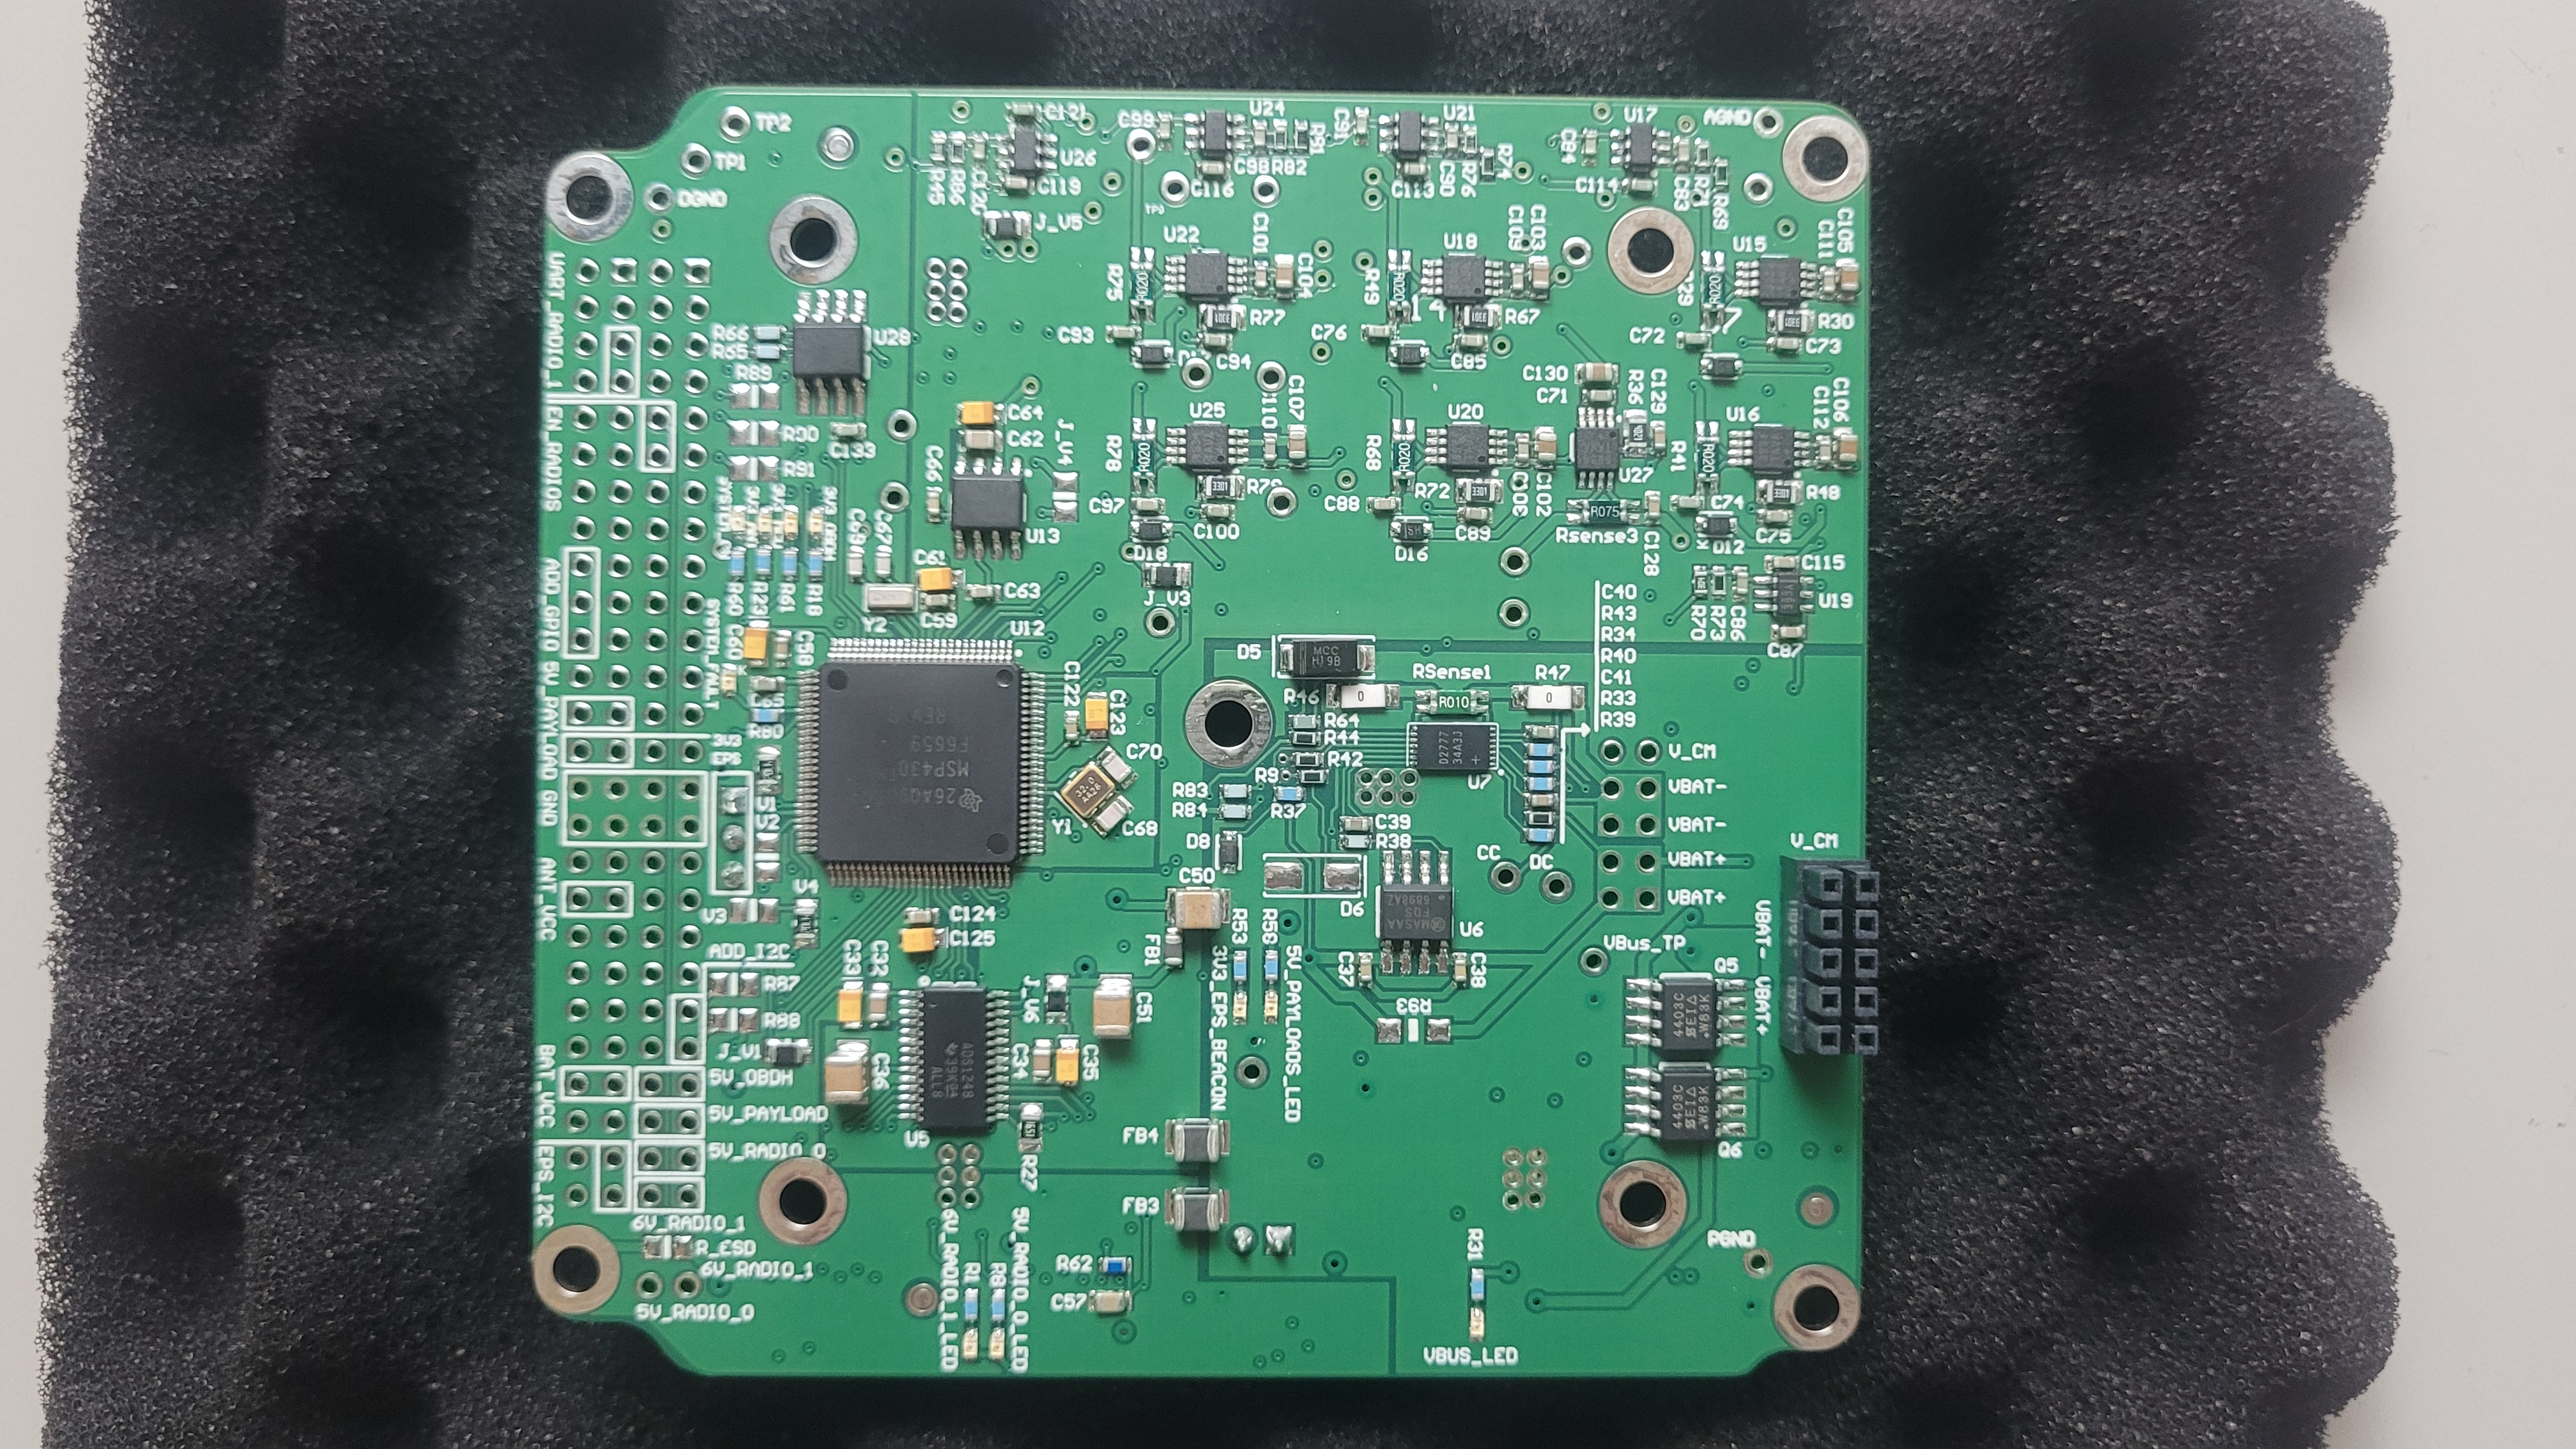
\includegraphics[width=0.6\textwidth, keepaspectratio]{figures/eps2_pcb_bottom.jpg}
    \caption{EPS 2.0 v0.3 bottom view.}
    \label{fig:eps2-pcb-bottom}
\end{figure}

The models were manufactured with the version v0.3 of the hardware design, found in the EPS 2.0 GitHub repository \cite{eps2-github}.
The manufacturer used was PCBWay, and the models were delivered in February, 2024.